\documentclass[tikz]{standalone}
\usepgflibrary{shapes.geometric}
\begin{document}
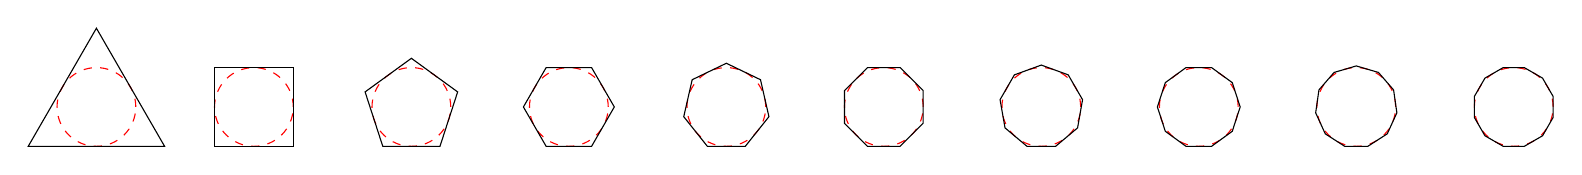
\begin{tikzpicture}
  \foreach \a in {3,...,12}{
	  \draw[red, dashed] (\a*2,0) circle(0.5cm);
	  \node[regular polygon, regular polygon sides=\a, draw,
	  inner sep=0.3535cm] at (\a*2,0) {};
	}
\end{tikzpicture}

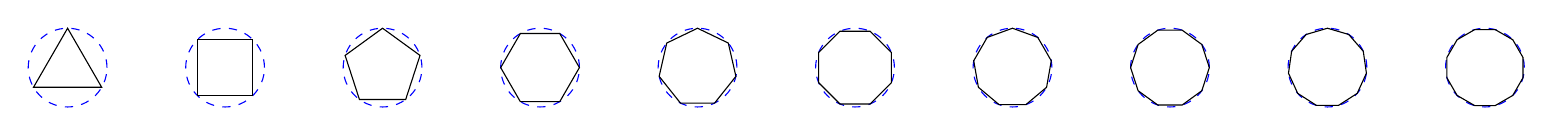
\begin{tikzpicture}
  \foreach \a in {3,...,12}{
	\draw[blue, dashed] (\a*2,0) circle(0.5cm);
	\node[regular polygon, regular polygon sides=\a, minimum size=1cm, draw] at (\a*2,0) {};
  }
\end{tikzpicture}

\end{document}
